\chapter{Bloqueadores de visibilidade}

Dados um conjunto de pontos $P$ em posição geral e um outro conjunto de pontos $B$. Dizemos que $B$ bloqueia a visibilidade de $P$ (ou só que $B$ bloqueia $P$) se para cada par $p_1,p_2$ de pontos de $P$ existir um ponto de $B$ no segmento aberto de $p_1$ a $p_2$. Vamos definir:

$$b(P) = min\{|B|:B\text{ bloqueia }P\}$$
$$b(n) = min\{b(P):|P|=n,P\text{ está em posição geral}\}$$

\cite{blockers} chegou a essas definições tentando provar a conjectura \ref{conj1} do capítulo anterior e tentou estimar o crescimento assintótico de $b(n)$.

\begin{conjectura}
    $$\frac{b(n)}{n}\rightarrow\infty$$

    Ou seja, $b(n)$ é superlinear
\end{conjectura}

São conhecidos limitantes inferiores lineares e limintantes superiores superlineares para $b(n)$, que serão mostrados na sessão seguinte.

\section{Ordem de crescimento de $b(n)$}

Dado um conjunto $P$ de pontos no plano, seja $\mu(P)$ a quatidade de pontos médios:
$$\mu(P)=|\{(\frac{(p+q)}{2}:p,q\in P, p\neq q\}|$$
E seja
$$\mu(n)=min\{\mu(P):|P|=n\}$$

Claramente $b(n)\leq \mu(n)$, pois o conjunto dos pontos médios é um conjunto bloqueador. Então vamos estimar $\mu(n)$.

\begin{teorema}
    $\mu(n)\leq ne^{C\sqrt{logn}}$ para alguma constante $C$. 
\end{teorema}
\begin{proof}

\end{proof}

\begin{corolario}
    $b(n)\leq ne^{C\sqrt{logn}}$ para alguma constante $C$. 
\end{corolario}

Matousek só conseguiu o seguinte limitante inferior trivial (\cite{blockers}), mas não houveram muitos avanços desde então, só uma pequena melhora por \cite{block}.

\begin{teorema}
    $b(n)\geq 2n-3$
\end{teorema}
\begin{proof}
    Se $P$ é um conjunto de $n$ pontos e $conv(P)$ tem $c$ pontos, uma triangulação de $P$ tem $3n-c-3$ segmentos de reta. Como precisamos de pelo menos um ponto para bloquear cada uma desses segmentos, temos que $b(P)\geq 3n-c-3\geq 2n-3$.
    \begin{center}
        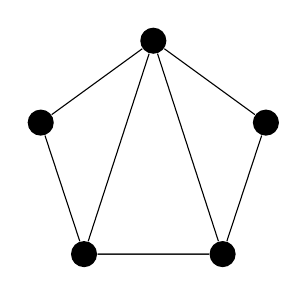
\begin{tikzpicture}
            \node[fill, circle] (V1) at (0,1.5) {};
            \node[fill, circle] (V2) at (1.43,0.46) {};
            \node[fill, circle] (V3) at (0.88,-1.21) {};
            \node[fill, circle] (V4) at (-0.88,-1.21) {};
            \node[fill, circle] (V5) at (-1.43,0.46) {};

            \draw[thin] (V1) -- (V2) -- (V3) -- (V4) -- (V5) -- (V1);
            \draw[thin] (V1) -- (V3)  -- (V4) -- (V1);
        \end{tikzpicture}
        
    Exemplo com $n=5$.
    \end{center}
\end{proof}

\cite{block} ainda mostrou que $b(n)\geq \frac{25}{8}n-o(1)$.

\section {Conjuntos em posição convexa}
Para conjuntos de pontos e posição estritamente convexa, pode-se obter resultados melhores. \cite{blockers} mostrou que, nesse caso, $b(P)=\omega(nlogn)$.

\begin{teorema}[\cite{blockers}]
Se $P$ é um conjunto de $n$ pontos em posição geral e estritamente convexa, então:

    $$b(P)\geq
    \begin{cases}
        n\sum_{k=0}^m\frac{1}{k} \text{ se }n=2m+1\text{ é ímpar}\\
        1+n\sum_{k=0}^m\frac{1}{k} \text{ se }n=2m\text{ é par}\\
    \end{cases}$$
\end{teorema}
\begin{proof}

\end{proof}

